\documentclass[12pt]{article}

\usepackage[utf8]{inputenc}
\usepackage{latexsym,amsfonts,amssymb,amsthm,amsmath}
\usepackage{float}

\setlength{\parindent}{0in}
\setlength{\oddsidemargin}{0in}
\setlength{\textwidth}{6.5in}
\setlength{\textheight}{8.8in}
\setlength{\topmargin}{0in}
\setlength{\headheight}{18pt}
\usepackage{graphicx}

\usepackage{caption}
\DeclareCaptionFormat{citation}{%
  \ifx\captioncitation\relax\relax\else
    \captioncitation\par
  \fi
  #1#2#3\par}
\newcommand*\setcaptioncitation[1]{\def\captioncitation{\textit{Source:}~#1}}
\let\captioncitation\relax
\captionsetup{format=citation,justification=centering}


\title{MATH1034OL1 Pre-Calculus Mathematics Notes from Sections 1.4, 1.7, 2.2, and 4.4}
\author{Elijah Renner}

\begin{document}

\maketitle

\vspace{0.5in}

\tableofcontents





\section{Reference Angles}
We define reference angles as the smallest positive acute angle formed by the terminal side of an angle and the x-axis on a coordinate plane:\\

\begin{figure}[ht]
	\centering
	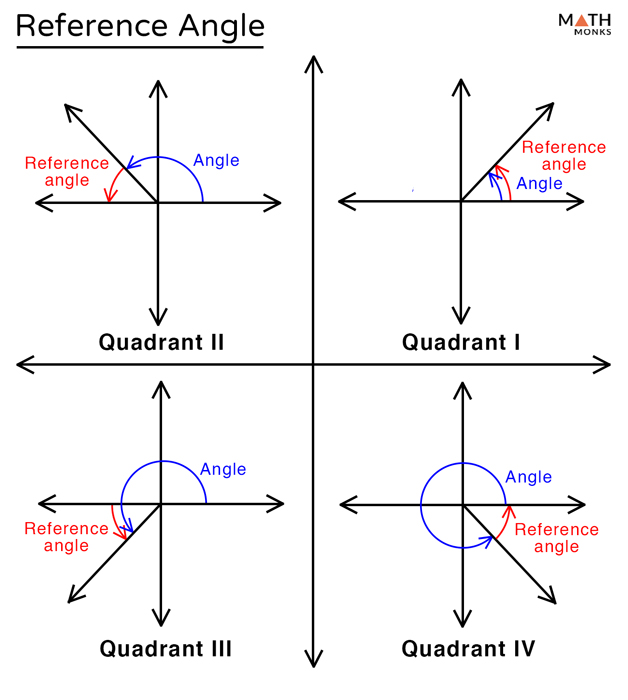
\includegraphics[scale=0.25]{Reference-Angle}
	\caption{Credit: https://mathmonks.com/angle/reference-angle}
\end{figure}

Imagine you're asked to evaluate \(\cos({\frac{7\pi}{6})}\). In order to do so, you must first find the reference angle. After we become more familiar with radian measures, it will be easy for you to determine that \(\frac{7\pi}{6}\) is in the third quadrant. However, until then, we can convert this measure to degrees: \\

\[\frac{7\pi}{6}\cdot\frac{180^{\circ}}{\pi}=210^{\circ}\]\\

If that didn't make sense, here are the methods for converting between radians and degrees:

% Conversion from degrees to radians
\[ \text{Radians} = \text{Degrees} \times \frac{\pi}{180} \]

% Conversion from radians to degrees
\[ \text{Degrees} = \text{Radians} \times \frac{180}{\pi} \]

In any case, now we can find our reference angle. Since the reference angle must be acute, we subtract \(180^{\circ}\): \(\text{reference angle}=210^{\circ}-180^{\circ}=30^{\circ}\). Now we can evaluate \(\cos({\frac{7\pi}{6})}\) using the 30-60-90 triangle.\\ 
\begin{figure}[ht]
	\centering
	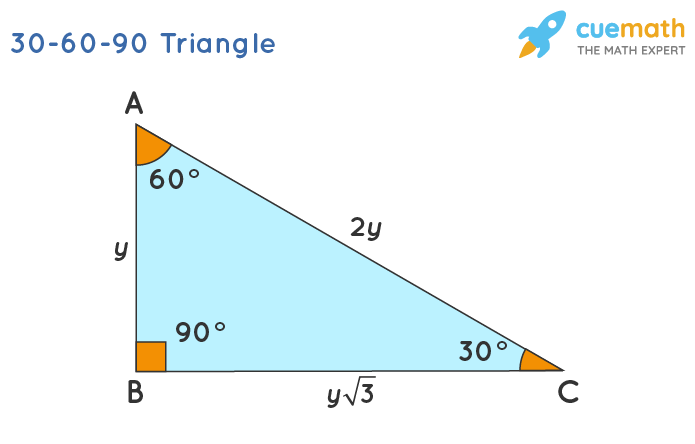
\includegraphics[scale=0.5]{30-60-90-triangle-1621153010}
	\caption{Credit: https://www.cuemath.com/geometry/30-60-90-triangle/}
\end{figure}

In the above figure, we assume \( y=\frac{1}{2} \) so that we interpret the angle as being on the unit circle (a circle with radius 1). We know that \(\cos \theta = \frac{\text{adjacent}}{\text{hypotenuse}}\). In our case, \(\text{adjacent} = \frac{\sqrt{3}}{2}\) and \(\text{hypotenuse} = 1\). If we plug these values into our cosine function, we see that \(\cos\left(\frac{7\pi}{6}\right) \neq \frac{\sqrt{3}}{2}\). \\

Huh? Am I crazy? Why did I put \(\neq\), you might ask? Well, it's because the value of \(\cos\left(\frac{7\pi}{6}\right)\) is actually negative. This makes sense because quadrant three is behind the y-axis, meaning that the adjacent side inherits a negative value. So, \(\cos\left(\frac{7\pi}{6}\right) = -\frac{\sqrt{3}}{2}\).\\

Also, did you catch the beauty of dealing with the unit circle? It's neat because, for sine and cosine, the values are easily found by referencing the two special triangles. We didn't need to perform any fraction division.\\

\section{Signs of Trigonometric Functions}

If that last part didn't make sense, don't worry. There's an incredibly simple way to remember this. Welcome ASTC or "All Students Take Calculus." It's an acronym that tells us which trig functions are positive in each quadrant.\\

\begin{figure}[ht]
	\centering
	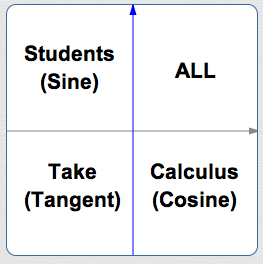
\includegraphics[scale=.75]{memoryDeviceSigns}
	\caption{Credit: https://www.onemathematicalcat.org}
\end{figure}

\section{Evaluating on Intervals and Solving for Variables in Trigonometric Equations}

Problem: find all the values \(t\) that satisfy \(\csc{t}=\sqrt{2}\) on the interval \([0,2\pi)\).\\

To find all values of \( t \) that satisfy \( \csc t = \frac{\sqrt{2}}{1} \) on the interval \( [0, 2\pi) \), follow these steps:

\subsection*{Step 1: Convert to Familiar Function}
\textbf{Convert to standard trig function:} \( \csc t = \frac{1}{\sin t} = \sqrt{2} \). This implies \( \sin t = \frac{1}{\sqrt{2}} = \frac{\sqrt{2}}{2} \).

\subsection*{Step 2: Identify Relevant Angles}
\textbf{Identify Relevant Angles:} Determine where \( \sin t = \frac{\sqrt{2}}{2} \). These angles are \( t = \frac{\pi}{4} \) and \( t = \frac{3\pi}{4} \).

\subsection*{Step 3: Check Interval}
\textbf{Check Interval:} Ensure that the angles \( \frac{\pi}{4} \) and \( \frac{3\pi}{4} \) are within the interval \( [0, 2\pi) \).\\

Since they do, \( \frac{\pi}{4} \) and \( \frac{3\pi}{4} \) are the values of \(t\) that satisfy our equation.\\

That's cool. Here's a harder one.\\

Problem: find all the values \(t\) that satisfy \(\sin{3t}=-\frac{\sqrt{3}}{2}\) where \(t\in[0,2\pi)\).\\

We begin by finding the values \(3t\) such that \(\sin3t=-\frac{\sqrt{3}}{2}\). Since \(-\frac{\sqrt{3}}{2}\) is negative, we know by our "All Students Take Calculus" that the solution(s) \(3t\) are in  quadrants three and/or four.\\

The sine value \(-\frac{\sqrt{3}}{2}\) tells us that the reference angle is part of a 30-60-90 triangle.\\

If you draw two 30-60-90 triangles on the unit circle in quadrants three and four, each having \(-\frac{\sqrt{3}}{2}\) as the long leg, the angles that form these triangles are:\\

\[\pi+\frac{\pi}{3}=\frac{4\pi}{3}\]
\[\pi+\frac{\pi}{2}+\frac{\pi}{6}=\frac{5\pi}{3}\]

So, \(3t=\frac{4\pi}{3}, \frac{5\pi}{3}\). But, remember, \(t\in[0,\pi)\). This means that

\[3t=\frac{4\pi}{3}+k2\pi \text{ for all \(k\in\{k | t<2\pi \text{ and } k\in\mathbb{Z}\}\)},\]

\[\frac{5\pi}{3}+k2\pi \text{ for all \(k\in\{k | t<2\pi \text{ and } k\in\mathbb{Z}\}\)}\]\\

Given this, we can test values k (or take more revolutions around the unit circle) to find all the values t that satisfy the equation.\\

Let's start with the first part, \(3t=\frac{4\pi}{3}+k2\pi\):

\[k=0: 3t=\frac{4\pi}{3}\implies \boxed{t=\frac{4\pi}{9}}\]

\[k=1: 3t=\frac{4\pi}{3}+2\pi\implies \boxed{t=\frac{10\pi}{9}}\]

\[k=2: 3t=\frac{4\pi}{3}+4\pi\implies \boxed{t=\frac{16\pi}{9}}\]

\(k\neq3\) because if \(k=3\) then \(t\notin[0,2\pi)\). Next, we find the coterminal angles of \(3t=\frac{5\pi}{3}+k2\pi\) such that \(t<2\pi\):

\[k=0: 3t=\frac{5\pi}{3}\implies \boxed{t=\frac{5\pi}{9}}\]

\[k=1: 3t=\frac{5\pi}{3}\implies \boxed{t=\frac{11\pi}{9}}\]

\[k=2: 3t=\frac{5\pi}{3}\implies \boxed{t=\frac{17\pi}{9}}\]

Again, \(k\neq3\) because if \(k=3\) then \(t\notin[0,2\pi)\).\\

Those are our solutions!

\section{Review of Linear Functions}

To find the slope of a line given two points, we use \(slope = m = \frac{\Delta y}{\Delta x}\). Given two points \((x_1,y_1) \text{ and } (x_2, y_2)\), we can calculate the slope using\\

\[\frac{y_1-y_2}{x_1-x_2}\]

If we a line's slope \(m\) and a point \((x_1,y_1)\) on the line, we can write its equation as\\

\[y-y_1=m(x-x_1)\]

Some rules:\\
A line parallel to a line with slope \(m\) will have slope \(m\)\\
A line perpendicular to a line with slope \(m\) will have slope \(-\frac{1}{m}\)\\
A line written in the form \(Ax+By=C\) will have slope \(m=-\frac{A}{B}\) and y-intercept \(b=\frac{C}{B}\)\\

\section{Properties of Graphs}

An axis of symmetry is defined as the line that divides the figure into two equal parts where one is the mirror image of the other.\\

\begin{figure}[H]
	\centering
	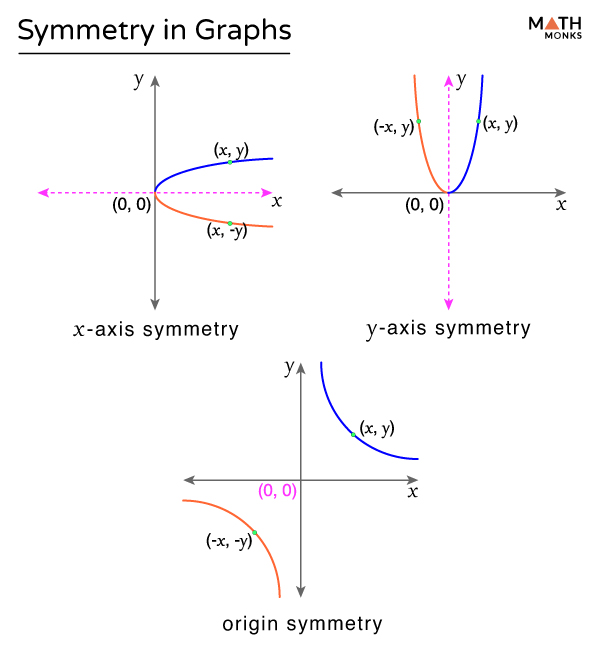
\includegraphics[scale=0.4]{Graph-Symmetry.jpg}
	\caption{Credit: https://www.cuemath.com/geometry/parabola/}
\end{figure}

\section{Absolute Value Equations}

\begin{figure}[H]
	\centering
	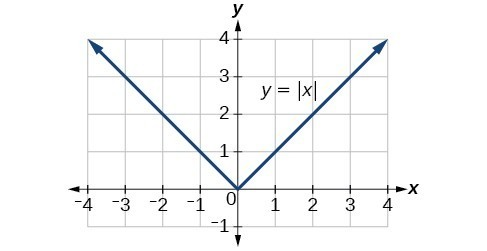
\includegraphics[scale=0.3]{CNX_Precalc_Figure_01_06_0032.jpg}
	\caption{Credit: https://courses.lumenlearning.com/ivytech-collegealgebra/chapter/graph-an-absolute-value-function/}
\end{figure}

\section{End Behaviors}

\begin{figure}[H]
	\centering
	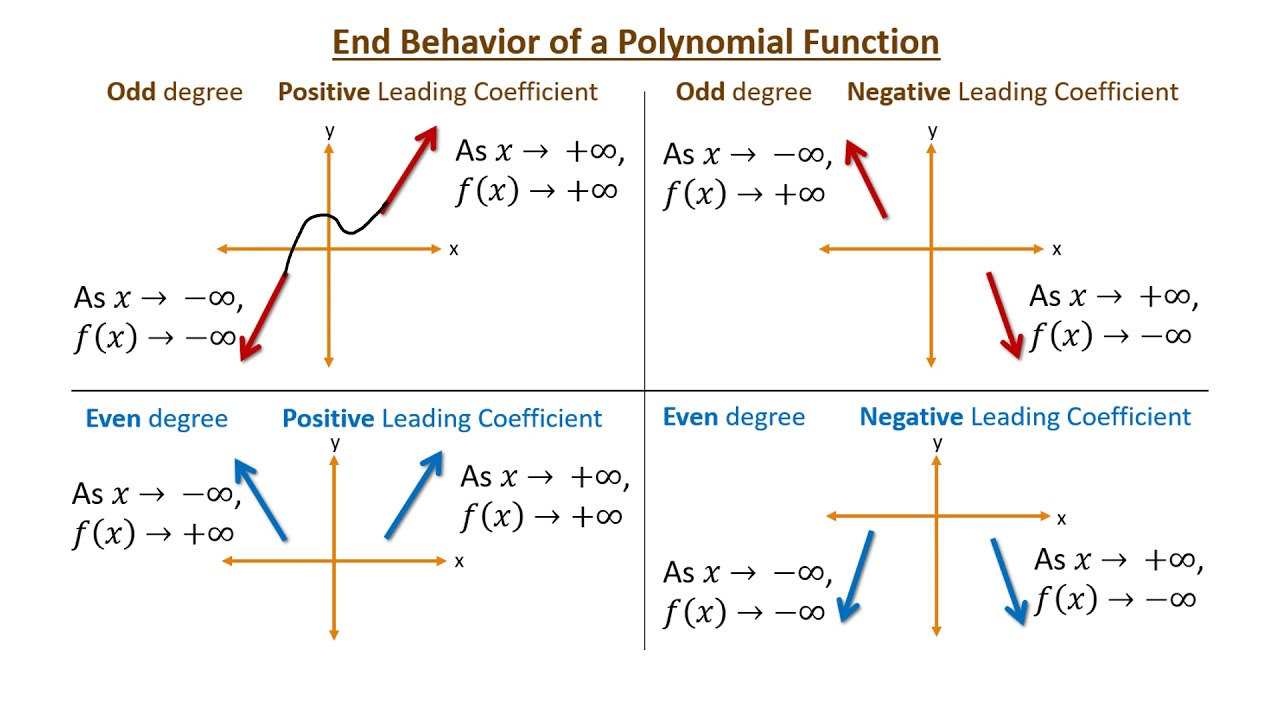
\includegraphics[scale=0.4]{maxresdefault.jpg}
	\caption{Credit: https://youtu.be/7LnsYtCfkXQ?si=Iq8WqdaHbLvWcLC0}
\end{figure}

\section{Transformations of Functions}

Here's a helpful graphic about transforming functions:

\begin{figure}[H]
	\centering
	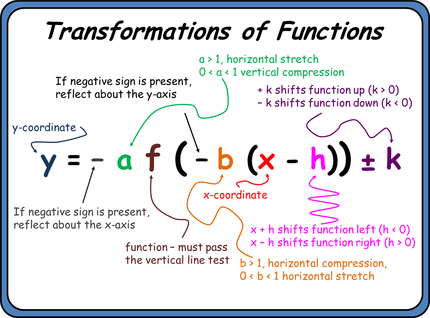
\includegraphics[scale=0.5]{9546920.png}
	\caption{Credit: https://lzinnick.weebly.com/transformations-of-functions-and-graphs.html}
\end{figure}



\end{document}
